\section{世界模型与可干预压缩}

形式要在哪里接受检验，行动又从哪里获得校正信号，这两个问题合起来指向一个被反复讨论却很少被准确定义的对象：世界模型。要理解这个词，先要绕开一个更常见的争论。关于人工智能，最容易陷入的争论之一，是追问它到底有没有“真正智能”。如果真正智能被定义为自主意识、自我目的、主体经验和类人式理解，那么这个问题很快会滑向哲学和科幻，这样的 AGI 是否会出现，何时出现，以何种形式出现，今天没有确定答案。但工程发展并不等待终极定义，飞机不是因为人类先理解了鸟类意识才飞起来，计算机也不是因为先拥有数学家的心灵才开始计算，现实中的技术路径，通常不是从终点倒推，而是从可用能力出发，在任务、工具和反馈中逐步扩展边界。从这个角度看，大模型首先不是一个完成的通用心灵，而是一种强大的模仿-压缩系统：它从海量文本、图像、代码和交互数据中学习模式，形成对语言、知识、风格、程序结构和任务关系的统计压缩，它的能力不是传统意义上的严格演绎，而是在巨大经验空间中进行相似性匹配、结构补全和概率生成。说它像一只越来越会说话的鹦鹉，并不完全错误，但这个比喻也容易遮蔽关键之处：当模仿足够深，覆盖足够广，并且接入工具、记忆、反馈和任务环境时，模仿就不再只是机械复述，而会成为一种可用的近似智能，模仿不是智能的终点，但可以成为闭环智能的起点。

\subsection{从模仿到可用近似：世界模型从哪里来}

\subhead{从模仿到可用近似}

人工智能史本身，就是对“智能如何获得世界”的反复试验。早期符号主义 AI 试图用形式逻辑和规则系统构造智能，它的理想很清楚：只要把世界写成命题、规则和推理链，智能就可以像数学证明一样展开。这一思路继承了更早的形式化冲动，世界可以被编码，推理可以被规则化，智能可以被还原为符号操作，它的深层假设是：如果世界可以被充分描述，智能就可以通过规则获得世界。但开放现实不是一个已经写完公理的封闭系统，规则越多，组合越复杂；目标越开放，语境越难穷尽；系统越接近现实，例外、噪声、身体、历史和后果就越无法被完整枚举。现实不是一张静态命题表，而是一个会被行动不断改变的过程，智能要进入这样的世界，不能只靠内部规则闭合，它必须把自身判断交给环境检验。现代神经网络选择了另一条路：它不从显式规则出发，而从数据分布中学习结构；不先写出世界的逻辑公理，而是通过拟合、压缩和泛化得到可用模式。CNN、Transformer 和各种深度网络都不是传统意义上的演绎机器，它们更擅长从大量样本中学会“像什么”“接下来可能是什么”“什么结构反复出现”，这条路不完美，容易幻觉，缺乏严格可证性，但它绕开了纯符号系统必须显式枚举世界的困难，不要求世界先被完整写成规则，才开始产生能力。

这条路线曾经被投入过极大的资源。日本在 1982 年启动第五代计算机计划，由通产省下属的新一代计算机技术研究所执行，十年间投入约五百七十亿日元，目标是造出一台以谓词逻辑推理为核心的高速并行推理机。计划在 1992 年按期结束，也演示了六十四处理器的并行原型，但没有带来工业界可以采用的产品，同期通用计算机的性能增长大幅压缩了专用推理机的价值空间\cite{aiso1988fifth,feigenbaum1993japanese}。这个案例说明的并不是规则系统没有能力，而是把世界显式写成规则这件事，其成本随覆盖范围增长得太快，而通用硬件和通用数据的收益又来得太快。

因此，大模型路径的核心价值，不在于它已经解决了终极理解问题，而在于它提供了一种现实可扩展的近似智能。它可以先模仿，再组合；先补全，再规划；先生成，再由外部反馈修正，它并不需要一开始就拥有完整世界模型，才可以产生价值，事实上，许多智能能力不是在封闭内部一次性形成的，而是在与外部环境反复耦合中逐步稳定。

\subhead{世界模型从哪里来}

这里就进入“世界模型”的问题。一种常见说法是：AI 必须先拥有世界模型，才可能获得真正智能。这个判断有道理，没有某种关于世界的内部结构，系统就无法预测后果、规划行动、区分表象与规律，也无法在不同情境中迁移经验，一个完全没有世界结构的系统，只能在输入和输出之间做局部反应，很难形成稳定行动。但这个判断立刻遇到一个反问：世界模型从哪里来？如果世界模型来自经验，那么经验必须通过感知、行动和反馈获得；如果世界模型需要反馈校正，那么系统必须先把自己的判断交给环境检验；如果世界模型要支持行动，那么行动又不能等到模型完全成熟之后才开始。系统必须在模型不完整时行动，又必须通过行动让模型变得更完整，它不能先站在世界之外，把世界完整建模，再回到世界中执行任务。这就是世界模型的循环依赖：没有模型，行动缺少方向；没有行动，模型缺少来源。模型需要行动来生成，行动又需要模型来引导，它们不是简单的先后关系，而是在同一个闭环中彼此塑形。这个闭环还有一个不可消除的时间方向：模型来自过去，是经验、数据和失败的压缩；行动面向未来，是对尚未出现后果的投注。低耦合任务之所以容易稳定，是因为未来大体可以由过去外推；强闭环任务之所以困难，是因为行动会改变后续条件；而反身高耦合任务之所以更难，是因为对象还会因模型、预测和干预而重新组织自己，使未来不再只是过去的延长。

但这里还隐藏着一个更深的误解。“世界模型”这个词，很容易让人以为智能内部应该有一张关于世界的地图：外部有一个世界，内部有一个模型，世界是被描述的对象，模型是对对象的表征，仿佛智能首先要在内部拥有一张较完整的地图，然后再拿着地图行动。可一个嵌入世界的行动者，并没有这种外部视角，它不是先站在世界之外，把世界完整拍成一张照片，再回到世界中执行计划，它从一开始就在世界之内，它的感知已经被身体位置、任务目标、工具接口、历史经验和行动能力塑形，它看到的不是纯粹世界，而是与自身可能行动相关的世界。因此，世界模型不是世界的照片，而是行动后果的压缩。智能真正需要的，不一定是一张关于世界的完整内部图像，而是对“如果我这样做，会发生什么”的预期结构：它需要知道哪些路径更可能成功，哪些动作会带来危险，哪些误差可以修正，哪些失败无法回滚。所谓模型，不是把世界搬进内部，而是在行动之前减少昂贵错误，在行动之后吸收反馈，在下一次行动中少撞一次墙。这也是大模型成功给我们的启发：它没有物理身体，也没有直接接触真实世界，却能通过对人类符号经验的压缩完成大量有用任务，这说明智能不一定从完整世界模型开始，很多时候，它从局部模式、任务结构、符号压缩和反馈修正开始，完整世界模型不是智能的前提，而可能是智能长期行动之后留下的沉积物。所以，真正的问题不应是：AI 是否已经拥有世界模型；更准确的问题是：一个智能系统在什么任务中，需要多强的模型-行动耦合。

\subhead{数字智能体与具身智能}

Agent AI 是这种逻辑在数字环境中的体现。单纯的大模型有明显边界：它可以生成文本和方案，但如果不能调用工具、观察结果、修正计划，它的能力就停留在一次性输出层面。Agent 系统把模型接入文件、浏览器、代码环境、数据库、软件界面和任务管理流程，让它可以分解目标、执行步骤、观察反馈、调整策略，模型不再只是回答问题，而是进入一个任务闭环：计划、行动、观察、修正、再行动。这并不意味着 Agent 立刻拥有真正自主智能，但它改变了能力结构，许多原本要求单次推理解决的问题，被转化为多轮试错和反馈控制问题，模型不必一次性正确，它可以通过环境反馈逐步逼近正确，它的有效智能，不只存在于模型参数内部，也分布在工具、接口、记忆、日志、测试和外部反馈之中，工具不是智能的附属装饰，而是智能闭环的一部分。这也是“世界模型从哪里来”这个问题的另一半答案：模型的一部分并不长在参数里，它长在工具链、日志和失败记录里，只要这些外部结构还在，模型就不必把全部世界装进自己。

具身智能面对的是同一类问题，只是介质更重。大模型目前主要从文本、图像、代码和人类知识中学习，它得到的是被人类表达过的世界，是二手经验、压缩经验和符号化经验。这已经非常强大，因为人类文明的大量知识都沉淀在符号中，但它仍然缺少许多一手反馈：触觉、力觉、空间连续性、物理接触、长期因果、行动后果。具身智能的价值，就在于把 AI 重新接回真实物理世界，让系统获得不只是关于世界的描述，而是在世界中行动后的后果。描述可以在符号空间中流畅展开，后果只能在世界中显现。一个模型可以生成关于杯子的文字，也可以识别杯子的图像，但真正拿起杯子时，它必须面对重量、摩擦、重心、接触角度、滑移、碰撞和反馈延迟；一个模型可以生成治疗建议，但药物进入身体后，会遇到吸收、代谢、免疫、毒性、个体差异和长期副作用；一个模型可以设计交通方案，但方案进入城市后，会遇到道路、产权、法规、习惯、事故责任和行为反应。模型如果不能穿过这些反馈，就只是关于世界的语言，而不是进入世界的能力。三者都说明模型必须穿过反馈，但反馈机制并不相同：杯子体现的是物理接触后的状态残差，药物体现的是生命系统的代谢、补偿和个体差异，交通方案体现的是制度、责任和行为反应，它们共同构成“进入世界”的阻力，不能被还原为同一种耦合。由此也可以理解，符号内部的自洽既强大又危险：大模型可以在语言中生成完整论证，也可以在风格、类比和概念之间形成高度一致性，但如果这种一致性缺少外部校正，它就可能把语言内部的顺滑误认为现实中的有效。它可以扩展可能性，却未必知道哪些可能性能够穿过现实阻力；它可以生成答案，却未必知道答案进入世界后会改变什么。

\subsection{耦合的三种强度、残差与反身}

\subhead{耦合的三种强度}

耦合可以分成三种工作情形。低耦合允许候选先被检查，输出不必立即改变外部状态；强物理闭环中，每次行动都会改变下一步遇到的对象；反身闭环中，其他行动者还会解释模型并调整策略。这些情形可以在同一系统内并存。社会系统可以形成稳定均衡，也可以持续漂移，不能由反身性直接断言没有不动点。

三种耦合在时间尺度上的差距可以量出来。工业机器人的伺服回路通常以千赫兹量级运行，电流环和位置环在毫秒量级完成一次修正；但接触任务真正可用的力控带宽要低一个数量级，常被传动柔性、传感安装、工件刚度和通信延迟压到十赫兹附近，继续调高增益只会激发未建模的振动\cite{eppinger1987}。而语言模型的一次输出延迟在数百毫秒量级。这意味着接触任务不能被处理成把大模型的输出直接接到伺服环上：语义判断可以慢，力和位置的回环必须快，中间必须有时间尺度转换，否则中耦合任务的残差会在两次模型输出之间滚出去很远。

\subhead{残差与反身}

世界模型的循环依赖并不是智能尚未成熟时的缺陷，而是智能嵌入世界后的基本状态。模型和行动不是两件先后发生的事，模型在行动中生成，行动在模型中获得方向，智能不是先拥有世界再行动，而是在行动中逐渐获得一个与自身相关的世界。这个闭环能否自举，取决于更新算子是否把偏差压回去：
\begin{equation}
\begin{split}a_t&=\pi(m_t),\quad m_{t+1}=U(m_t,a_t)=F(m_t),\\ DF(m)&=\frac{\partial U}{\partial m}+\frac{\partial U}{\partial a}D\pi(m).\end{split}
\end{equation}
$m_t$为模型状态，$a_t$为行动。稳定性需要考察复合映射$F$，第二项保留“模型改变行动，行动再改变更新”的路径。若$F$把一个完备的不变域映入自身，并在其中一致压缩，则迭代收敛到该域内唯一不动点。单点导数或局部线性化只提供局部判断，环境变化、噪声与延迟还会改变结果。SLAM展示了边走边建模的可行路线，实际收敛仍依赖可观测性、传感与运动条件。

但具身智能的真正难处，比建图更深。SLAM 默认地图大体稳定，你测量它，它不会因为被测量而主动改变自身，这个例子说明世界模型可以在稳定对象中通过自举逐步形成，但它还没有触及行动的全部重量。物理操作中的杯子、地面和身体，也不会因为被建模而主动改变，它们真正的困难在于，一旦被接触，就会留下后果：机器人一接触杯子，杯子的位置、姿态、摩擦状态和后续可抓取性就已经改变；一次脚步失稳，身体姿态和地面接触已经改变；一次夹持过重，物体可能变形或破裂。这里的问题不是对象会读懂模型，而是行动会改写下一步初始条件。这就是中耦合任务的困难：世界不会主动反身，但行动会留下残差，行动之后，原来的建模对象虽然没有“逃避”模型，却已经不在原来的状态中。因此，具身智能的典型困难还不是高反身耦合，而是强物理闭环耦合，杯子不会预判机器人，地面不会理解算法，门把手不会围绕模型改变策略，但它们会在接触中改变状态，并把这种改变带入下一步行动，只有当任务环境中包含人、组织、交通参与者或其他会解释并回应模型的行动者时，具身智能才进一步进入反身高耦合，一般物理对象不会回应模型，但会被行动改写，这已经足以构成具身智能的核心困难。它不是在静止世界中建模，而是在被自己行动持续改写的世界中继续行动。

物理世界不会在每一步之后自动回到原点。文本可以重写，代码可以回滚，图像可以再生成，但物理动作会留下后果：一次小的识别误差会改变抓取姿态，一次接触偏差会改变物体位置，一次控制延迟会放大下一步规划误差，残差不会在动作之间自动清零，而会沿任务链滚动。具身智能真正要处理的，不是静态世界的完整描述，而是行动之后仍能继续行动的后果管理。这也是为什么世界模型不能被理解为一个孤立模块，仿佛只要把它造出来，智能就自然出现：真正有用的世界模型，不只是描述对象，而是管理后果，它既来自观察，也来自行动；既来自预测，也来自预测失败之后的修正；既要压缩过去经验，也要追踪自己对世界造成的改变。它不是外部观察者画出的完整图册，而是行动者在不断介入世界之后留下的可行动压缩。

\subhead{耦合的台阶与后果管理}

从技术黏滞的角度看，世界模型问题揭示的不是“模型越来越重”这么简单，而是模型-行动耦合会发生类型变化。比特域允许低成本生成和回滚，模型可以相对轻；原子域的行动会留下不可自动清零的残差，模型必须接入反馈；生命系统会通过代谢、补偿、适应和个体差异改变干预后果；社会系统则会解释、回应、套利甚至反抗干预，使模型本身成为系统动态的一部分。这里不是一个单纯“耦合越来越强”的连续旋钮，而存在一道台阶：中耦合面对的是被行动改写的对象，高耦合面对的是会回应模型的对象，前者的核心问题是残差滚动，后者的核心问题是反身漂移。世界越重，模型越不能只是描述；对象越会回应模型，模型越不能假装自己站在世界之外。因此，真正重要的问题不是“AI 有没有世界模型”，而是“它的模型在何种介质中，以何种方式与行动耦合”：低耦合任务允许模型像语言一样流动，强物理闭环耦合任务要求模型在行动中在线校正，追踪自身行动留下的残差，反身高耦合任务则让模型成为世界动态的一部分。世界模型不是一个统一物件，而是一组随任务、介质、后果强度和对象反身性变化的行动预期结构。

这也让“循环依赖”获得了新的意义。循环依赖不是一个需要被彻底克服的缺陷，而是智能嵌入世界后的常态：模型不是行动之前的纯粹图像，行动也不是模型之后的机械执行，模型在行动中被证明，也在行动中失效；行动由模型引导，也反过来改变模型要面对的世界。智能不是摆脱这个循环，而是学会在循环中保持可修正、可恢复、可继续行动。所以，具身智能真正需要的不是一张终极地图，而是对后果的持续校正：它不必拥有完整世界，才能开始行动；但它必须知道自己的行动如何改变下一步世界；它不必把全部现实装进内部模型；但它必须在相关任务中维持行动与反馈之间的稳定关系。失败不是因为没有全知模型，而是因为行动之后的世界偏离了系统能够继续处理的范围。这条判断也有边界：如果某类任务中的输出几乎不改变下一轮对象，错误可以低成本回滚，反馈可以被外部筛选，那么世界模型可以保持较弱、较松、较符号化；反之，如果一个系统越行动，后续状态越被自身改写，残差越沿任务链滚动，失败越难恢复，那么它就越需要强模型-行动耦合。此时，所谓世界模型不能被理解为静态内部表征，而应被理解为行动后果的在线压缩。

由此看，AGI 也许不该被想象成某个突然降临的完整主体。更现实的路径，是许多能力在闭环中逐步拼合：语言模型提供符号压缩，Agent 系统提供任务执行，工具环境提供外部记忆和计算，具身系统提供物理反馈，长期交互提供因果数据，验证机制提供纠错约束，智能不是从单点爆发，而是在多个闭环中逐渐形成更大的可行动结构。这条路径不浪漫，但更真实，它不要求系统一开始就有完整意识，也不要求它先验掌握世界本体，它只要求系统能够在有限模型下行动，在行动中获得反馈，在反馈中修正模型，在修正后扩大行动范围。大模型像不像鹦鹉，并不是最关键的问题，关键在于，这只“鹦鹉”是否被接入了工具、记忆、反馈、身体和真实任务：如果它只在笼子里重复语言，它当然主要是模仿；如果它能通过行动获得反馈，修正自身计划，并把失败转化为下一步调整，它就开始进入智能发展的自举通道；如果它还能处理自身行动对世界造成的改变，追踪被自己改写过的对象，它才真正进入具身智能的核心区域。世界模型的根本困难，不只是世界太大，也不只是模型太弱，而是“世界模型”这个说法本身容易让人忘记：智能从来不是在世界之外拥有世界，它只能在世界之内，通过行动获得后果，通过后果修正自身，通过修正后的自身再次行动。智能不是先拥有世界再行动，而是在行动中获得世界，但它获得的那个世界，已经被自己的行动改变过。

\subsection{可干预压缩：因果与尺度的门槛}

模型必须从世界的反应中学习，这句话说起来简单，做起来要回答一个更早的问题：什么样的压缩才算抓住了世界的反应。压缩在这里不是数据处理的技巧，而是有限智能面对世界时的基本处理方式，它决定了模型能在多大范围内保持可用。由此出现一个更具体的问题：压缩到什么程度才算抓住了世界的反应，而不只是记住了世界的痕迹。大模型使一个旧问题重新变得尖锐：如果智能是一种压缩，而真实世界本身也充满概率，那么概率模型能不能表征世界？答案不能简单地说能或不能。概率不是障碍，量子测量、热噪声、混沌系统和有限观测都说明，世界在许多尺度上只能以概率方式被描述，真正的问题不是模型是否使用概率，而是这种概率是否受到现实约束；不是它能否生成合理延续，而是它能否在行动之后仍然预测世界怎样反应。\key{大模型主要学习世界留下的痕迹，世界模型的门槛在于学习世界对干预的反应。}痕迹可以复制、重放、切片、标注和反复训练；反应必须通过接触世界获得，并带有成本、延迟、噪声、风险和不可逆性。文本、图像、视频和代码都是世界的痕迹，它们来自经验、观察、制度、叙事、实验和操作，但它们不是世界本身，模型可以从这些记录中恢复出大量结构，却不能因此自动获得改变现实系统的能力。

\subhead{可干预压缩}

压缩不是大模型的技巧，而是有限智能面对世界时的基本处理。真实世界的状态空间无法被完整复制，有限智能也不保存世界的高清副本，它只能在任务、误差和风险要求下，动态选择需要保留、忽略或重新观察的变量：粒子、材料、边界、历史路径、噪声、他者行动和结构耦合同时存在，任何行动都只能在极小的切片中发生，智能不是把世界装进内部，而是在不可复制的世界中选择少数对行动有用的状态变量，没有这种选择，就没有感知、概念、因果、规划和行动。所谓\term{可干预压缩}，不是把世界完整压缩进模型，而是在无法复制整个状态空间的条件下，对世界反应进行粗粒化：删去当前尺度下不支配状态转移的细节，保留那些在干预、边界变化和反事实比较中仍然有效的变量。粗粒化不是随意简化，而是为了行动而选择有效变量，删去当前任务中不改变结果的细节，保留会改变状态转移的结构，世界模型因此不是世界的副本，而是在特定尺度、任务和边界条件下有效的行动模型。

观察、干预和反事实的区分，在因果推断中已有明确框架。\cite{pearl2009causality} 记录可以包含实验和机制知识，模型也可能从记录中学到因果结构；预测记录准确，却不自动证明某项现实干预可靠。可干预压缩要求把这种可靠性落实到指定任务、尺度与反馈上。

\subhead{因果与尺度}

因果在这里出现。世界模型需要的不是所有共同变化，而是在干预下仍然改变状态转移的结构：相关性告诉模型什么经常一起出现，因果告诉模型改变什么会改变结果。药物不保证每个人必然有效，但它改变疗效和副作用的概率分布；控制信号不保证机器人每次轨迹完全一致，但它改变状态转移的方向，因果不是确定性链条，而是行动系统在压缩世界反应时必须保留的最低结构。因果还要求反事实和尺度选择：行动者不只要知道“做 A 会怎样”，还要比较“不做 A、做 B、稍后做、换一种方式做”会带来哪些不同结果，没有反事实，就没有规划、纠错和责任判断；因果变量也不是固定的，分子尺度、机械尺度、任务尺度和组织尺度各有不同的因果结构，世界模型的困难，不是把所有相关线索都当成原因，而是找出当前尺度上真正改变状态转移的变量。

保留哪些变量、删去哪些变量，可以写成一个判据
\begin{equation}
\left|\frac{\partial f}{\partial x_i}\right|\sigma_i>\theta
\end{equation}
$f$ 是状态转移函数，$x_i$ 是候选状态变量，$\sigma_i$ 是该变量在当前任务与时间窗内的典型涨落幅度；$\partial f/\partial x_i$ 是状态转移对它的敏感度，两者之积是变量涨落可能造成的状态转移变化量，与容限 $\theta$ 同量纲；$\theta$ 是任务允许的状态转移误差，因此判据本身是一次无量纲比较。满足判据的变量进入模型，不满足的被压缩掉，这正是前一段所说“删去不支配状态转移的细节、保留在干预下仍然有效的变量”的写法。判据依赖任务、时间尺度、风险等级和耦合范围，所以可干预压缩没有绝对正确的粒度，只有相对于这些条件的最小充分粒度：尺度太粗，模型看不见真正改变结果的变量；尺度太细，模型被无关细节淹没，失去行动能力。这个粒度也不是行动前就能完全求出的答案，而是在建模、试探、失败和修正中逐步逼近的边界。

这也意味着，因果结构并不总能以清晰、稳定、低维的形式出现。在强噪声、强混沌或不可约随机的尺度上，微小扰动可能被迅速放大，单次结果可能无法精确预测，所谓“支配状态转移的变量”也未必能被压缩成简单关系，此时，世界模型能够保留的不是确定链条，而是概率约束、鲁棒边界和风险分布。可干预压缩并不假定世界处处存在可完全掌握的因果结构，它只要求模型在给定任务和尺度下，尽可能保留那些仍能改变结果分布、限制状态转移或界定失败风险的结构，概率不是因果的反面，在许多现实系统中，因果只能以概率形式被保留。所以，好的世界模型不是知道得最多，而是知道哪些东西在当前尺度上不能忽略。抓取杯子时，分子细节通常可以删去，摩擦和重心不能删去；研究材料疲劳时，微裂纹不能删去；预测拥堵时，个体神经活动可以删去，群体流量和反应延迟不能删去。这里也不能把模式和约束简单对立：约束不是模式的反面，而是在情境改变、尺度变化和行动干预下仍然限制状态转移的稳定结构，高频模式告诉模型通常会发生什么，约束告诉模型在什么边界内仍然成立，什么情况不可能成立，越界后会怎样失败，一个模型如果只学会表象中的高频模式，却没有学会限制状态转移的结构，就可以生成合理画面，却不能稳定指导现实行动。

\subhead{前沿路线与共同门槛}

视频模型、交互式模型、视觉—语言—动作系统、仿真训练与在线反馈，都在连接记录和行动反应。Google DeepMind在2026年7月的Gemini Robotics 2工作中进一步结合全身动作与高层能力。\cite{geminirobotics2026} 需要检查的共同接口是任务、硬件、反馈、恢复与泛化证据。

但这也暴露出同一个底层问题：记录可以被复制，反应必须被支付。文本、图像、视频和演示轨迹可以大规模重放，真实行动后的世界反应却带有成本、延迟、噪声、风险和不可逆性。仿真可以降低试错成本，但不能取消仿真与现实之间的偏差\cite{tobin2017domain}。奖励可以推动策略优化，但不能保证覆盖长期风险；在线交互可以暴露错误，但在原子、生命和社会系统中，许多错误本身就是代价。世界模型的门槛不在表象是否连贯、环境是否可交互、动作接口是否完整，而在模型能否用有限、昂贵、带风险的世界反应，形成可推广、可验证、可承担的行动判断。

压缩还受到可逆性的限制。被删去的变量如果可以重新观测，压缩风险较低；如果只能通过昂贵试错恢复，风险就会上升；如果行动发生后状态无法恢复，就不能轻易删除。比特空间中的错误常常可以撤销，原子、生命和社会系统中的错误则可能留下不可逆后果。可干预压缩不是尽可能删去变量，而是在错误可恢复性、验证成本和后果不可逆性之间决定删去多少。这三项条件共同决定了同一个判据在不同介质中的门槛：同样是抓取，在仿真环境中删去接触细节的代价接近于零，在真实产线上删去接触细节的代价可能是撞坏工件或伤及人员。

\subhead{黏滞与世界反应}

这正是技术黏滞展现的地方。世界反应不是免费反馈，而是被资源、时间和结构过滤过的反馈：资源约束决定一次真实反应需要支付多少能量、材料、空间、算力、设备、维护和冗余成本；时间约束决定反应何时出现，是否存在不可压缩的等待、老化、训练、反馈和恢复周期；结构约束决定局部动作会如何穿过耦合网络，被放大、抵消、绕回或锁死。技术黏滞不是世界模型之外的阻力，而是世界反应本身的成本结构，真正的世界模型，不是世界外观的生成器，而是在资源、时间与结构约束下判断状态转移的有效模型。

在高耦合和多智能体系统中，问题还会进一步加深。世界不只是被动回应行动，其他行动者会根据模型的行动重新调整自己的预期、策略和约束，此时，模型要校准的不再是固定环境中的状态转移，而是会因自身介入而改变的反应分布。模型一旦进入系统，就成为系统的一部分，它对世界的预测会改变世界对它的反应，这正是上一节所说的反身漂移在世界模型问题中的表现，可干预压缩在这里最容易失效，因为被压缩的对象不是静态环境，而是会回应、会学习、会反过来改变模型输入的结构。

验证不是世界模型的外部补丁，而是现实对错误压缩的反作用机制：任何压缩都会丢失信息，关键在于被丢掉的信息是否会在行动中重新变得重要。失败不是压缩的偶然事故，而是压缩边界的展现，机器人抓取失败，说明某个被忽略的接触、摩擦、姿态或传感变量重新出现；自动驾驶失误，说明某个罕见场景、遮挡关系、意图判断或反馈延迟不能被压缩掉；药物失效或产生毒性，说明某条代谢路径、剂量关系或长期作用没有被模型保留。压缩负责删去变量，现实会让被错误删去的变量重新展现出来。

这也是世界模型必须进入闭环的原因。封闭语料中的概率分布，只能反映世界曾经如何被记录；行动闭环中的概率分布，才开始反映世界如何回应干预。模型每一次行动，都会把内部压缩暴露给外部现实；现实每一次反馈，都会迫使模型修正状态变量的选择。学习世界不是一次性获得完整图景，而是在干预、失败、修正和再压缩中，逐渐找到足以行动的结构，世界模型不是静态知识库，而是由世界反应持续校准的状态转移模型。因此，可干预压缩可以定义为：智能系统在无法复制整个状态空间、也无法无限试错的条件下，把世界对干预的反应粗粒化为一组仍能稳定判断状态转移、约束边界、反事实后果和失败模式的变量、关系与结构。这个定义不试图取代世界模型，而是说明世界模型进入现实系统时必须满足什么条件，它必须在有限、昂贵、带风险的反应中保留足够可靠的行动结构。真正与真实相反的，不是概率，而是没有被世界反应校准的概率；真正与行动相反的，不是压缩，而是不能承受干预检验的压缩。

\subhead{有限反应中的行动判断}

大模型证明了一件重要的事：世界留下的痕迹可以被学习到惊人的程度。世界模型还要证明另一件更难的事：它能否只靠有限、昂贵、带风险的世界反应，学到一个经得起推敲的行动判据。前者发生在符号、图像和视频的延续中，后者发生在干预、代价、失败和修正中。真正的跃迁，不是从概率走向非概率，而是从学习世界留下的痕迹，走向学习世界对行动的反应。记录可以教会模型世界如何被说出，反应才能教会模型世界如何被改变。智能要进入现实，不能只学习世界如何被描述，还必须学习世界如何被改变。

反应的价格可以按医药研发的账本来估。DiMasi、Grabowski 和 Hansen 在 2016 年基于十家药企的一百零六个新药样本给出的估计是，一个获批新药的自付研发支出平均约十三点九五亿美元，按百分之十点五的实际折现率资本化到获批时点，总额约二十五点五八亿美元\cite{dimasi2016}。进入临床的化合物最终获批的比例通常在百分之十上下，中枢神经系统药物还要更低。这些数字对应的是同一件事：记录可以被无限次复制，一次真实反应却要按项目、按年份、按失败率支付，而且支付之后不一定换来可用的结论。

但一旦问题落到这里，讨论的对象就不再只是模型。反应要靠身体去接触世界，残差也要靠身体去吸收。压缩判据决定了模型保留哪些变量，而身体决定了这些变量在接触中由谁修正、以多大延迟修正、失败之后能否恢复。同一个判据在模型内部是可以计算的，在物理接触中却要由材料、结构和反射来承担，这就是形态计算传统要处理的问题。身体只是这类承载结构中的一层。在远比它更长的时间尺度上，还有一层结构在做同样的事：它不靠传感器和反射，而靠世代更替来记录哪些变量不能删去，靠繁殖失败来确认哪些压缩是错的。它的验证周期以代计，它的错误不能回滚，它的变量一旦写进去，就要在接下来的所有行动中持续支付。要判断智能在物理介质中能走多远，就必须先看清这套更古老的压缩机制是怎么运转的。


\begin{figure}[ht]
\centering
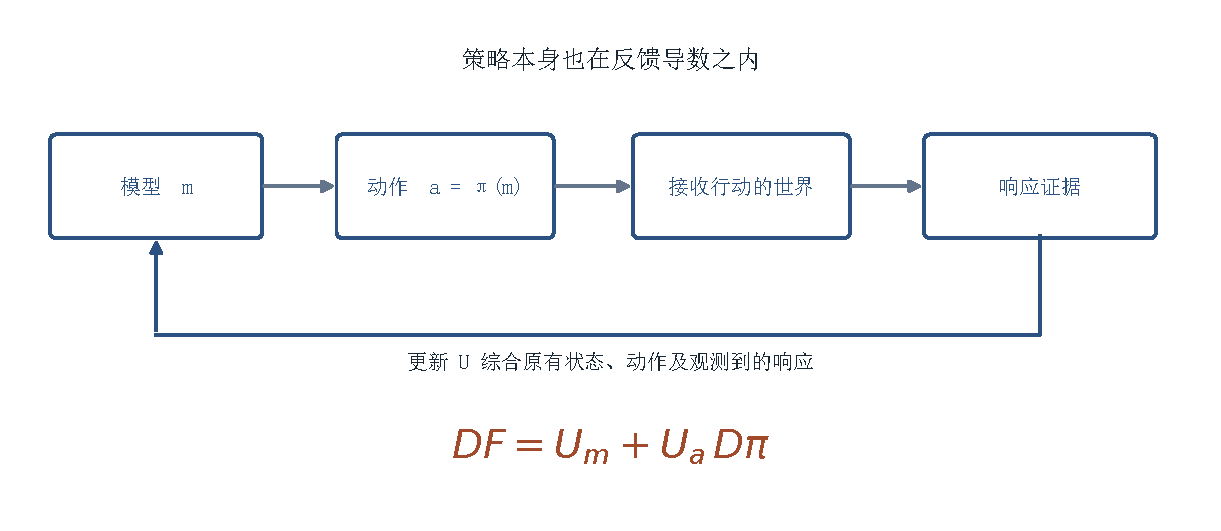
\includegraphics[width=\textwidth]{figures/model-action-loop.pdf}
\caption{模型通过策略改变动作，动作又改变下一次更新的证据。$U$综合保留状态、动作与环境响应，复合映射的导数同时包含直接项与经由策略的间接项。}
\label{fig:mechanism-model-action-loop}
\end{figure}
\furtherreading{%
W. Brian Arthur，\textit{The Nature of Technology: What It Is and How It Evolves}\\
Thomas P. Hughes，\textit{Rescuing Prometheus: Four Monumental Projects That Changed the Modern World}\\
Per Bak，\textit{How Nature Works: The Science of Self-Organized Criticality}\\
Sidney Dekker，\textit{Drift into Failure: From Hunting Broken Components to Understanding Complex Systems}\\
Stewart Brand，\textit{How Buildings Learn: What Happens After They’re Built}\\
Andy Clark，\textit{Surfing Uncertainty: Prediction, Action, and the Embodied Mind}\\
Sebastian Thrun, Wolfram Burgard and Dieter Fox，\textit{Probabilistic Robotics}\\
Judea Pearl and Dana Mackenzie，\textit{The Book of Why: The New Science of Cause and Effect}}


% <<<<<<<<<< parts/book-ch03.tex <<<<<<<<<<


% >>>>>>>>>> parts/book-ch04.tex >>>>>>>>>>
%% ===================== 本章参考文献 =====================
\printbibliography[heading=subbibliography,title=参考文献]
